\documentclass[a4paper, 11pt, oneside]{article}

\usepackage[utf8]{inputenc}
\usepackage[T1]{fontenc}
\usepackage[french]{babel}
\usepackage{array}
\usepackage{shortvrb}
\usepackage{listings}
\usepackage[fleqn]{amsmath}
\usepackage{amsfonts}
\usepackage{fullpage}
\usepackage{enumerate}
\usepackage{graphicx}             % import, scale, and rotate graphics
\usepackage{float}               
\usepackage{subfigure}            % group figures
\usepackage{alltt}
\usepackage{url}
\usepackage{indentfirst}
\usepackage{eurosym}
\usepackage{listings}
\usepackage{color}
\usepackage[table,xcdraw,dvipsnames]{xcolor}

% Change le nom par défaut des listing
\renewcommand{\lstlistingname}{Extrait de Code}

% Change la police des titres pour convenir à votre seul lecteur
\usepackage{sectsty}
\allsectionsfont{\sffamily\mdseries\upshape} 
% Idem pour la table des matière.
\usepackage[nottoc,notlof,notlot]{tocbibind} 
\usepackage[titles,subfigure]{tocloft} 
\renewcommand{\cftsecfont}{\rmfamily\mdseries\upshape}
\renewcommand{\cftsecpagefont}{\rmfamily\mdseries\upshape} 

\definecolor{mygray}{rgb}{0.5,0.5,0.5}
\newcommand{\coms}[1]{\textcolor{MidnightBlue}{#1}}

\lstset{
    language=C, % Utilisation du langage C
    commentstyle={\color{MidnightBlue}}, % Couleur des commentaires
    frame=single, % Entoure le code d'un joli cadre
    rulecolor=\color{black}, % Couleur de la ligne qui forme le cadre
    stringstyle=\color{RawSienna}, % Couleur des chaines de caractères
    numbers=left, % Ajoute une numérotation des lignes à gauche
    numbersep=5pt, % Distance entre les numérots de lignes et le code
    numberstyle=\tiny\color{mygray}, % Couleur des numéros de lignes
    basicstyle=\tt\footnotesize, 
    tabsize=3, % Largeur des tabulations par défaut
    keywordstyle=\tt\bf\footnotesize\color{Sepia}, % Style des mots-clés
    extendedchars=true, 
    captionpos=b, % sets the caption-position to bottom
    texcl=true, % Commentaires sur une ligne interprétés en Latex
    showstringspaces=false, % Ne montre pas les espace dans les chaines de caractères
    escapeinside={(>}{<)}, % Permet de mettre du latex entre des <( et )>.
    inputencoding=utf8,
    literate=
  {á}{{\'a}}1 {é}{{\'e}}1 {í}{{\'i}}1 {ó}{{\'o}}1 {ú}{{\'u}}1
  {Á}{{\'A}}1 {É}{{\'E}}1 {Í}{{\'I}}1 {Ó}{{\'O}}1 {Ú}{{\'U}}1
  {à}{{\`a}}1 {è}{{\`e}}1 {ì}{{\`i}}1 {ò}{{\`o}}1 {ù}{{\`u}}1
  {À}{{\`A}}1 {È}{{\`E}}1 {Ì}{{\`I}}1 {Ò}{{\`O}}1 {Ù}{{\`U}}1
  {ä}{{\"a}}1 {ë}{{\"e}}1 {ï}{{\"i}}1 {ö}{{\"o}}1 {ü}{{\"u}}1
  {Ä}{{\"A}}1 {Ë}{{\"E}}1 {Ï}{{\"I}}1 {Ö}{{\"O}}1 {Ü}{{\"U}}1
  {â}{{\^a}}1 {ê}{{\^e}}1 {î}{{\^i}}1 {ô}{{\^o}}1 {û}{{\^u}}1
  {Â}{{\^A}}1 {Ê}{{\^E}}1 {Î}{{\^I}}1 {Ô}{{\^O}}1 {Û}{{\^U}}1
  {œ}{{\oe}}1 {Œ}{{\OE}}1 {æ}{{\ae}}1 {Æ}{{\AE}}1 {ß}{{\ss}}1
  {ű}{{\H{u}}}1 {Ű}{{\H{U}}}1 {ő}{{\H{o}}}1 {Ő}{{\H{O}}}1
  {ç}{{\c c}}1 {Ç}{{\c C}}1 {ø}{{\o}}1 {å}{{\r a}}1 {Å}{{\r A}}1
  {€}{{\euro}}1 {£}{{\pounds}}1 {«}{{\guillemotleft}}1
  {»}{{\guillemotright}}1 {ñ}{{\~n}}1 {Ñ}{{\~N}}1 {¿}{{?`}}1
}
\newcommand{\tablemat}{~}

%%%%%%%%%%%%%%%%% TITRE %%%%%%%%%%%%%%%%
\newcommand{\facultee}{\textit{Premier bachelier en sciences informatique}}
\newcommand{\annee}{\textit{Année académique 2018-2019}}
\newcommand{\intitule}{\textsc{\textbf{INFO0030: Mastermind}}}
\newcommand{\GrNbr}{11}
\newcommand{\PrenomUN}{Marco}
\newcommand{\NomUN}{Naa}
\newcommand{\PrenomDEUX}{Jordi}
\newcommand{\NomDEUX}{Hoorelbeke}
\renewcommand{\tablemat}{\tableofcontents}

\title{\facultee \\ \annee \\ \intitule}
\author{Groupe \GrNbr : \PrenomUN~\textsc{\NomUN}, \PrenomDEUX~\textsc{\NomDEUX}}
\date{\today}

\begin{document}
\maketitle
\newpage
\tablemat
\newpage

%%%%%%%%%%%%%%%% RAPPORT %%%%%%%%%%%%%%%
\section{Introduction}
Dans le cadre du cours INFO0030: Projet de programmation, il nous a été demandé de réaliser le jeu Mastermind.
Ce rapport traitera:
\begin{itemize}
	\item[$\bullet$] L'architecture générale du code: les grands concepts et comment ils interagissent entre eux.
	\item[$\bullet$] La description des structures de données du code et leur pertinence.
	\item[$\bullet$] L'idée derrière certains algorithmes du code. Plus particulièrement,
	\begin{itemize}
	    \item[$\star$] L'algorithme qui compare la réponse et la proposition faite pour en retourner un score.
	    \item[$\star$] L'algorithme qui permet à l'ordinateur de faire sa proposition. 
	\end{itemize}
	\item[$\bullet$] Un profiling du code: le temps d'exécution des algorithmes importants et une estimation de la quantité de mémoire utilisée par les structures de données.
	\item[$\bullet$] L'organisation de l'interface graphique.
	\item[$\bullet$] L'utilisation du SCM et la coopération au sein du groupe
	\item[$\bullet$] Les amélioration possibles au jeu.
	\item[$\bullet$] La conclusion: ce que ce projet nous a apporté.
\end{itemize} 
\section{Architecture générale du code}
Le code suit le pattern MVC.
L'utilisateur interragit avec le contrôleur qui lui gère ces interractions et définit le comportement du jeu Mastermind. Le contrôleur implémente le modèle et la vue.
La vue quant à elle contient les labels et les images, c'est à dire tous les éléments qui vont être affichés à l'écran, hormis les boutons. La vue implémente le modèle.
Pour finir, le modèle contient toutes les fonctionnalités et algorithmes du jeu qui s'occupent des opérations internes.

Trois modes de jeu sont jouables:
\begin{itemize}
    \item[$\bullet$] Le mode humain (normal) qui se joue avec les règles classiques du Mastermind.
    \item[$\bullet$] Le mode humain (facile) qui est une version simplifée du Mastermind.
    \item[$\bullet$] Le mode ordinateur où c'est l'ordinateur qui doit déchiffrer votre combinaison de couleurs.
\end{itemize}

\section{Structures de données}
Différentes structures de données ont été implémentées:
\begin{itemize}
    \item[$\bullet$] La structure \textbf{Ordi} contient tous les outils supplémentaires nécessaires pour l'algorithme de l'ordinateur.
    \item[$\bullet$] La structure \textbf{Combinaison} représente une combinaison de couleurs et contient donc les informations d'ordre et de couleur des pions. La taille d'une combinaison de couleurs dépend de la macro NB\textunderscore COULEUR et est donc facilement paramétrable.
    \item[$\bullet$] La structure \textbf{Historique} contient l'historique des combinaisons réalisées lors d'une partie que ce soit dans le mode humain ou le mode ordinateur.
    \item[$\bullet$] La structure \textbf{Records} contient les outils suplémentaires nécessaires pour les records.
    \item[$\bullet$] La structure \textbf{ModeleMastermind}, l'implémentation du modèle du jeu et qui contient, entre autre, les structures Ordi, Combinaison, Historique et Records.
    \item[$\bullet$] La structure \textbf{VueMastermind}, l'implémentation de la vue du jeu et qui contient la structure ModeleMastermind ainsi que les labels et le chemin vers les images.
    \item[$\bullet$] La structure \textbf{ControleurMastermind}, l'implémentation du contrôleur du jeu et qui contient les structures VueMastermind et ModeleMastermind ainsi que les boutons. 
\end{itemize}
Le coût en terme de mémoire de ces structures sera abordé dans la section "Profiling et analyse de performance du code".

\section{Algorithmes particuliers}
Nous avons voulu mettre en avant deux algorithmes, ceux qui sont les pièces maitresses de notre code et qui nous ont pris le plus de temps. Il s'agit de notre algorithme comparant une proposition à la réponse pour fournir le score associé qui figure dans la fonction compare\textunderscore reponse\textunderscore proposition() et aussi à celui présent dans la fontion algorithme\textunderscore ordinateur() qui fournit la proposition de l'ordinateur en fonction des scores des précédentes manches.
\subsection{compare\textunderscore reponse\textunderscore proposition()}
Soit un tableau score de taille NB\textunderscore PIONS.
Cette proçédure compare la réponse cachée et la proposition faite par le devinant et place le score correspondant dans le tableau score. L'algorithme se déroule comme suit:
\begin{itemize}
    \item[$\bullet$] Initialisation de deux tableaux copieRep et copieProp de taille NB\textunderscore PIONS.
    \item[$\bullet$] Copiage de la réponse dans copieRep et de la proposition dans copieProp.
    \item[$\bullet$] Dans une première boucle, les deux tableaux sont comparés et lorsque dans ces deux tableaux au même indice se trouve la même couleur, les valeurs de ces deux cases sont affectées à zero\footnote{Mettre la valeur de ces cases à zero permet de ne plus les prendre en compte lors de la prochaine boucle qui compte le nombre de pions blancs et donc d'éviter d'avoir trop de pions blancs} et la couleur noir est mise dans le tableau score au même indice.
    \item[$\bullet$] Dans la deuxième boucle, grâce à une boucle imbriquée qui lit les valeurs du tableau copieProp, on compare les valeurs différentes de zéro de copieProp et celles de copieRep et quand ce sont les mêmes valeurs, un pion blanc est placé à une case égale à 0 dans le tableau score.
\end{itemize}

\subsection{algorithme\textunderscore ordinateur()}
L'algorithme de cette proçédure se déroule selon les règles suiventes:

Soient un tableau temporaire de taille NB\textunderscore PIONS, couleur la couleur courante, pionNoirs le nombre de pions noirs de la manche courante, pionBlancs le nombre de pions blancs de la manche courante, pion\textunderscore noir \textunderscore prec le nombre de pions noirs de la manche précédente et pion\textunderscore blanc\textunderscore prec le nombre de pions blancs de la manche précédente.

\begin{itemize}
    \item[$\bullet$] A la première manche, une couleur aléatoire est mise dans couleur et à chaque nouvelle manche, une couleur différente de celles déjà utilisées est mise dans couleur.
    \item[$\bullet$] Si pionNoirs + pionBlancs est plus grand que pion\textunderscore noir\textunderscore prec + pion\textunderscore blanc\textunderscore prec:
    \item[]Déplacer (pionBlancs-1) fois les cases du tableau contenant une valeur différentes de zéro avec ces trois règles:
    \begin{itemize}
        \item[$\star$] Parcourir le tableau par la gauche.
        \item[$\star$] Une case contenant une valeur différente de zéro peut être déplacée si et seulement si la valeur de la case à sa droite est zéro.
        \item[$\star$] Si on arrive à la fin du tableau et que la valeur de (pionBlancs-1) cases n'ont pas encore été déplacées alors recommencer dès le début du tableau.
    \end{itemize}
    \item[] Finalement, ajouter la/les nouvelles valeurs à la/les première(s) case(s) égale(s) à zéro à partir de la droite.
    \item[$\bullet$] Si pionBlancs + pionNoirs est égal à pion\textunderscore noir\textunderscore prec + pion\textunderscore blanc\textunderscore prec:
    \begin{itemize}
        \item[$\star$] Même chose que pour le point précédent sauf qu'on décale de pionBlancs fois les cases.
        \item[$\star$] Décaler la valeur de la case dans la première case valant zéro en allant vers la droite. Si aucune case égale à zéro n'est trouvée avant la fin du tableau, recommencer du début.
    \end{itemize}
\end{itemize}


\newpage
\section{Profiling et analyse de performance du code}
\subsection{Estimation de la quantité de mémoire utilisée par les structures de données}
La taille de nos structures est mesurée en octets,
Voici la liste des structures et leur taille en considérant que notre constante NB\textunderscore PIONS valait 4 :
\begin{itemize}
    \item[$\bullet$] La structure ModeleMastermind comprend:
\begin{itemize}
        \item[$\star$] CouleurProposition = \textbf{32 octets}
        \item[$\star$] Couleurscore = \textbf{12 octets}
        \item[$\star$] Combinaison = \textbf{34 octets}
        \item[$\star$] Ordi = \textbf{24 octets}
        \item[$\star$] Historique = \textbf{196 octets}
        \item[$\star$] Records = \textbf{52 octets}
        \item[$\star$] ModeFacile + ModeOrdinateur + Manche + CouleurCourante = \textbf{16 octets} 
        \item[$\star$] Tab\textunderscore imageP = \textbf{200 octets}
    \end{itemize}
    Ce qui nous fait un total de \textbf{566 octets} pour notre structure ModeleMastermind.
    \item[$\bullet$] La structure VueMastermind comprend:
    \begin{itemize}
        \item[$\star$] une structure ModeleMastermind = \textbf{566 octets}
        \item[$\star$] pLabelManche + pLableMode = \textbf{16 octets}
        \item[$\star$] imageP = \textbf{50 octets}
        \item[$\star$] imageS = \textbf{50 octets}
    \end{itemize}
    Ceci nous fait alors un total pour Vue de \textbf{682 octets}
     \item[$\bullet$]La structure ControleurMastermind comprend:
    \begin{itemize}
        \item[$\star$] une structure ModeleMastermind et une structure VueMastermind = \textbf{682 octets}
        \item[$\star$] pBoutonProposition = \textbf{320 octets}
        \item[$\star$] pBoutonScore = \textbf{320 octets}
        \item[$\star$] pBoutonCouleur = \textbf{56 octets}
        \item[$\star$] pBoutonOrdi = \textbf{32 octets}
        \item[$\star$] pBoutonOK = \textbf{8 octets}
        \item[$\star$] nb\textunderscore boutons\textunderscore clicked = \textbf{2 octets}
    \end{itemize}
\end{itemize}
    Le total pour Controleur et donc pour nos structures est donc de \textbf{1420 octets}.
\subsection{Temps d'exécution de diverses situations de jeu}
Les résultats suivants ont été obtenus grâce à la librairie standard time.h.
Avec la fonction clock(), le temps a été récolté au début et à la fin de diverses fonctions et la différence entre ces deux temps a donné les temps d'exécutions. \footnote{Chaque temps est une moyenne des différents temps récoltés sur plusieurs essais.}
\subsubsection{Dans le mode de jeu humain}
\begin{itemize} 
    \item[$\bullet$] Lorsque l'utilisateur appuie sur le bouton "nouveau" pour recommencer une partie, le temps d'exécution est d'approximativement \textbf{0.06 secondes}.
    \item[$\bullet$] Lorsque l'utilisateur appuie sur le bouton pour entrer une proposition, le temps d'exécution est d'approximativement \textbf{0.002 secondes}
    \item[$\bullet$] Lorsque l'utilisateur appuie sur le bouton OK pour valider sa combinaison, le temps d'exécution est d'approximativement \textbf{0.003 secondes} dont \textbf{0.002 secondes} pour l'algorithme qui se charge de calculer et d'afficher le score.
\end{itemize}

\subsubsection{Dans le mode de jeu ordinateur}
\begin{itemize}
    \item[$\bullet$] Lorsque l'utilisateur appuie sur le bouton "nouveau" pour recommencer une partie, le temps d'exécution est d'approximativement \textbf{0.05 secondes}.
    \item[$\bullet$] Lorsque l'utilisateur appuie sur le bouton OK pour voir la combinaison faite par l'ordinateur et le score associé, le temps d'exécution est d'approximativement \textbf{0.14 secondes} dont \textbf{0.000009 secondes} pour l'algortihme de l'ordinateur.
\end{itemize}

\section{Interface graphique du jeu}
En haut se trouve le menu du jeu Mastermind permettant d'acceder aux différentes options telles que:
\begin{itemize}
    \item[$\bullet$] \textbf{Partie}: 
    \begin{itemize}
        \item[$\star$] \textbf{Nouveau}: permet de lancer une nouvelle partie.
        \item[$\star$] \textbf{Records}: permet d'accéder aux dix meilleurs scores.
        \item[$\star$] \textbf{Quitter}
    \end{itemize}
    \item[$\bullet$] \textbf{Mode}:
        \begin{itemize}
            \item[$\star$] \textbf{Proposant: Humain(facile)}: Un mode de jeu facile où l'humain est le proposant et où le score s'affiche dans l'ordre.
            \item[$\star$] \textbf{Proposant: Humain(normal)}: Un mode de jeu normal où l'humain est le proposant et où le score s'affiche dans le désordre.
            \item[$\star$] \textbf{Proposant: Ordinateur}: Un mode où le proposant est l'ordinateur.
        \end{itemize}
    \item[$\bullet$] \textbf{Aide}:
    \begin{itemize}
        \item[$\star$] \textbf{A propos}: Ouvre une fenêtre POPUP contenant les informations sur les auteurs du jeu ainsi que le cours pour lequel il a été fait.
        \item[$\star$] \textbf{Règles du jeu}
    \end{itemize}
\end{itemize} 

En dessous du menu: 
\begin{itemize}
    \item[$\bullet$] Deux labels vous permettent de savoir dans quel mode et à quelle manche vous êtes et vous donne aussi le score une fois la partie terminée.
    \item[$\bullet$] La zone à gauche permet au devinant de faire ses propositions.
    \item[$\bullet$] La zone à droite affiche le score de chaque proposition.
    \item[$\bullet$] La zone du bas à trois utilitées:
        \begin{itemize}
            \item[$\star$] Sélectionner une couleur.
            \item[$\star$] Entrer une combinaison de couleurs que l'ordinateur devra déchiffrer.
            \item[$\star$] Valider sa proposition et/ou passer à la manche suivante en appuyant sur le bouton OK.
        \end{itemize}
\end{itemize}

\begin{figure}[H]
    \center
        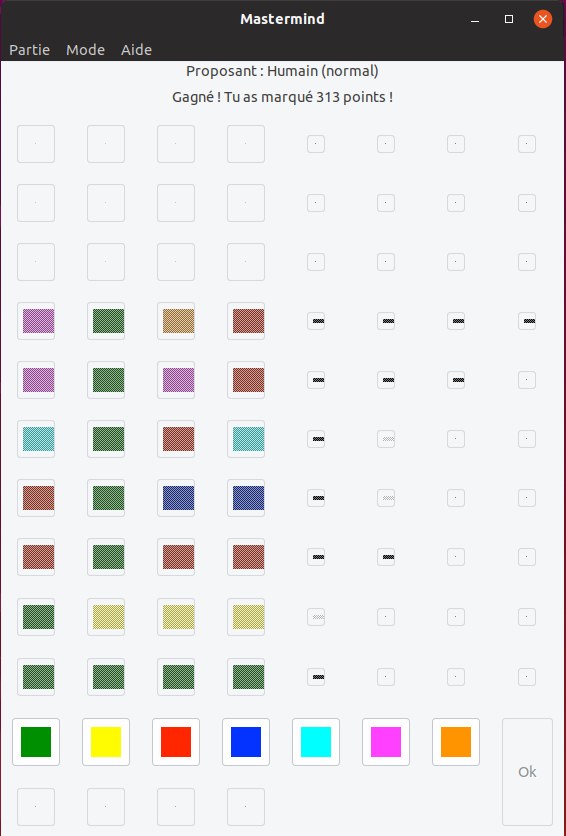
\includegraphics[scale=0.3]{images_rapport/proposanthumain.png}  
        \caption{Interface graphique du mode Proposant Humain}
\end{figure}

\begin{figure}[H] 
    \center
        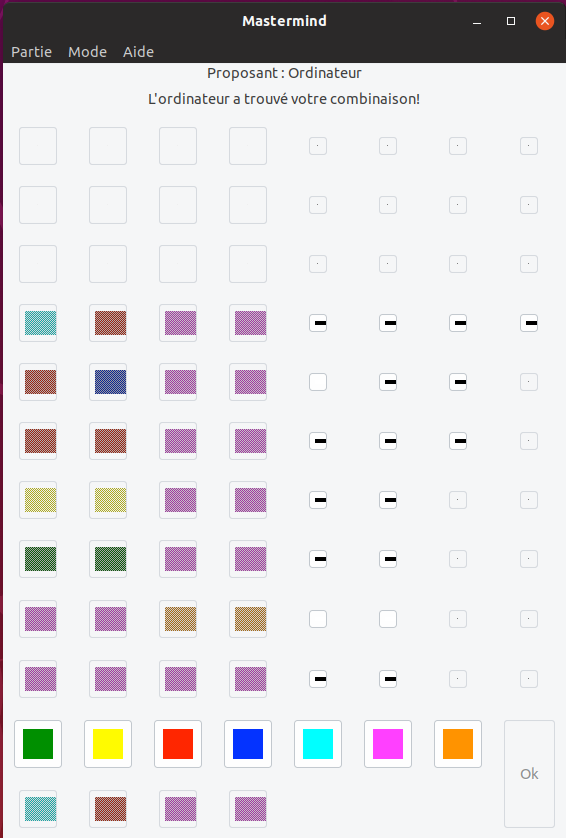
\includegraphics[scale=0.3]{images_rapport/proposantordi.png}
        \caption{Interface graphique du mode Proposant Ordinateur}
\end{figure}
\begin{figure}[H] 
    \center
        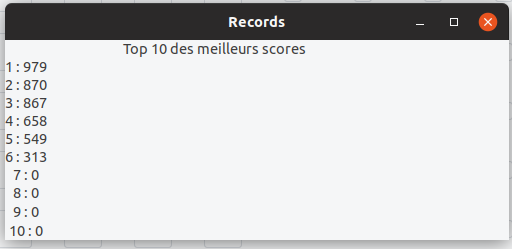
\includegraphics[scale=0.5]{images_rapport/records.png}  
        \caption{Boite de dialogue "Records"}
\end{figure}
\begin{figure}[H] 
    \center
        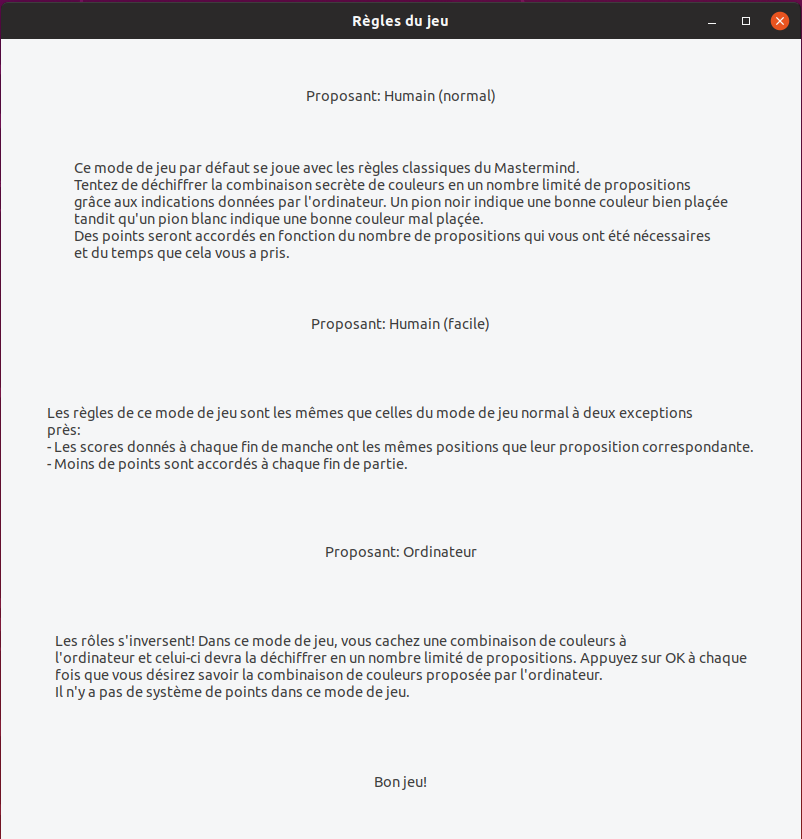
\includegraphics[scale=0.3]{images_rapport/reglesdujeu.png}  
        \caption{Boite de dialogue "Règles du jeu"}
\end{figure}
\begin{figure}[H] 
    \center
        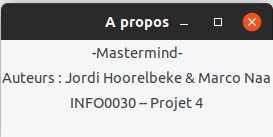
\includegraphics[scale=0.7]{images_rapport/apropos.png}  
        \caption{Boite de dialogue "A propos"}
\end{figure}



\section{Gestion du code et coopération au sein du groupe}
Pour la gestion du code cela s'est passé comme suit :
\begin{itemize}
    \item[$\bullet$] Nous avons d'abord discuté de l'architecture générale de notre code puis réalisé un plan afin de mieux organiser notre travail.
    \item[$\bullet$] Ensuite, nous avons mis en place les structures et le pattern MVC ce qui nous a servi de base pour notre codage.
    \item[$\bullet$] Pour les grands axes du code, notamment l'interface graphique de la fenêtre et les algorithmes complexes tels que les fonctions compare\textunderscore reponse\textunderscore proposition() et algorithme\textunderscore ordinateur(), nous nous sommes retrouvés à l'université afin de pouvoir y réflechir ensembles avant de pouvoir les implémenter.
    \item[$\bullet$] Les fonctions "secondaires" telles que toutes les fonctions callback ainsi que le calcul et le tri des scores ont quant à elles pu être codées puis implémentées chacun de notre coté avant d'être mises sur Gitlab. 
\end{itemize}
Le SCM nous à surtout été utile pour fusionner nos codes et pour retracer l'origine d'un problème quand il y en avait. Peut de temps avant la deadline du projet, nous nous sommes rendu compte d'un problème d'accès illégal à la mémoire qui empêchait le jeu de fonctionner. En retrouvant la dernière version du code source qui n'avait pas ce problème et en le comparant avec le code source le plus récent, il nous à été plus facile de localiser l'origine de ce problème.
\section{Améliorations possibles du code}
On pourrait apporter des améliorations dans notre code, notamment l'algorithme pour que l'ordinateur trouve une combinaison de couleur donnée pourrait être plus performant.
Actuellement et selon les divers tests que nous avons pu faire, cet algorithme trouve la solution dans \textbf{81\% des cas}, et ce après en moyenne \textbf{6,2 manches} pour les parties réussies, nous pouvons donc en conclure que cet algorithme est améliorable.
En plus de ça, de la même façon que nous avons implémenté un mode facile lorsque le proposant est l'être humain, nous pourrions implémenter un mode difficile où les propositions vides sont acceptées.

\section{Conclusion}
Pour conlure, nous pouvons dire que ce projet nous a permis de nous rendre compte à quel point il fallait être rigoureux dans l'implémentation du code pour que celui-ci fonctionne. Il nous a aussi appris à faire un plan avant de s'attaquer au codage car dans les grands fichiers il est souvent dur de s'y retrouver lorsqu'on est mal organisé et que faire un bon plan c'est déjà faire une bonne partie du travail, cela nous a aussi aidé à gérer notre temps car cela a été un des grands problèmes. A l'aide d'outils comme Gitlab, Codeshare/Collabedit et Overleaf, nous avons appris à coopérer et à travailler ensembles. Pour terminer, nous avons aussi vu que la pratique était le meilleur moyen de progresser en programmation.

\end{document}